% =====================================================================
% FRONT MATTER (Cluster A Sequence 1..14)
% =====================================================================

% 1. OUTER LAMINATED COVER (No page number, header or footer)
\thispagestyle{klfront}
\begin{center}
  \vspace*{-10mm}
  
\includegraphics[width=0.46\textwidth]{kl_logo_1.jpeg}\\[3mm]

  {\fontsize{14.5}{17}\selectfont\bfseries\color{KLDarkBlue} KONERU LAKSHMAIAH EDUCATION FOUNDATION}\\
  {\fontsize{10.5}{13}\selectfont\color{KLSlate} (DEEMED TO BE UNIVERSITY)}\\[1.5mm]
  {\fontsize{11.5}{14}\selectfont\bfseries\color{KLSlate} KLEF COLLEGE OF ENGINEERING}\\[4mm]

  {\fontsize{11.5}{14}\selectfont\bfseries\color{KLBlue} CLUSTER A --- SOFTWARE SYSTEMS ENGINEERING}\\[3mm]
  {\fontsize{17}{20}\selectfont\bfseries\color{KLDarkBlue} FINAL PROJECT REPORT}\\[4mm]

  {\fontsize{15}{19}\selectfont\bfseries\color{KLDarkBlue} Scalable Association-Rule Mining Estimator with Apriori Baseline (\skarm)}\\[5mm]

  {\fontsize{10.5}{14}\selectfont\color{KLMuted} A Final Project Report submitted in partial fulfilment of the requirements\\
  for the award of the degree of}\\[2mm]
  {\fontsize{12}{15}\selectfont\bfseries\color{KLSlate} BACHELOR OF TECHNOLOGY IN COMPUTER SCIENCE AND ENGINEERING}\\[5mm]

  {\fontsize{10.5}{13}\selectfont\itshape\color{KLMuted} Submitted by}\\[2mm]
  {\fontsize{10.5}{14.5}\selectfont\bfseries\color{KLSlate}
  Gontla Venkata Anvitha --- 2300032207\ \ $|$\ \ Abhishek Kumar --- 2300033822\\
  Kamma Giridhar --- 2300030295\ \ $|$\ \ Paladagula Venkata Rajeev --- 2300030497}\\[4mm]

  {\fontsize{10.5}{13}\selectfont\itshape\color{KLMuted} Under the supervision of}\\[2mm]
  {\fontsize{11}{14}\selectfont\bfseries\color{KLSlate} Dr.~Dudigam Ramya, [DESIGNATION], Dept.\ of CSE}\\[4mm]
\end{center}

\begin{klbox}
\fontsize{9.5}{13}\selectfont
\textbf{\color{KLBlue} Project identity:} Portal use-case ID: \textbf{KLCAP-2026-00340}\ \ $|$\ \ Team No.: \textbf{C2C-25}\ \ $|$\ \ Approved cluster: \textbf{Cluster A --- Software Systems Engineering}\ \ $|$\ \ Dominant specialization: \textbf{AI for Computational Intelligence}
\end{klbox}

\vfill
\begin{center}
  {\fontsize{10.5}{13.5}\selectfont\bfseries\color{KLSlate} DEPARTMENT OF COMPUTER SCIENCE AND ENGINEERING}\\
  {\fontsize{10}{13}\selectfont\color{KLMuted} Green Fields, Vaddeswaram -- 522 502, Andhra Pradesh, India}\\[1.5mm]
  {\fontsize{10.5}{13.5}\selectfont\bfseries\color{KLSlate} November, 2026\ \ $|$\ \ Academic Year 2026--27}
\end{center}

% 2. INNER TITLE PAGE (No page number, header or footer)
\newpage
\thispagestyle{klfront}
\begin{center}
  \vspace*{-10mm}
  
\includegraphics[width=0.40\textwidth]{kl_logo_1.jpeg}\\[2.5mm]
  {\fontsize{13.5}{16}\selectfont\bfseries\color{KLDarkBlue} KONERU LAKSHMAIAH EDUCATION FOUNDATION}\\
  {\fontsize{10}{12.5}\selectfont\color{KLSlate} (DEEMED TO BE UNIVERSITY)}\\[3.5mm]

  {\fontsize{14.5}{18}\selectfont\bfseries\color{KLDarkBlue} Scalable Association-Rule Mining Estimator with Apriori Baseline (\skarm)}\\[3.5mm]

  {\fontsize{10}{13}\selectfont\color{KLMuted} A Final Project Report submitted in partial fulfilment of the requirements for the award of the degree of}\\
  {\fontsize{11.5}{14}\selectfont\bfseries\color{KLSlate} BACHELOR OF TECHNOLOGY IN COMPUTER SCIENCE AND ENGINEERING}\\[3mm]

  {\fontsize{10}{12.5}\selectfont\itshape\color{KLMuted} by}\\[1.5mm]
  {\fontsize{10.5}{14}\selectfont\bfseries\color{KLSlate}
  Gontla Venkata Anvitha (2300032207)\ \ $|$\ \ Abhishek Kumar (2300033822)\\
  Kamma Giridhar (2300030295)\ \ $|$\ \ Paladagula Venkata Rajeev (2300030497)}\\[3mm]

  {\fontsize{10}{12.5}\selectfont\itshape\color{KLMuted} under the supervision of}\\
  {\fontsize{11}{14}\selectfont\bfseries\color{KLSlate} Dr.~Dudigam Ramya, [DESIGNATION]}\\
  {\fontsize{9.5}{12.5}\selectfont\color{KLMuted} Department of Computer Science and Engineering}
\end{center}

\vspace{1mm}
\begin{center}
\fontsize{9.5}{12.5}\selectfont
\resizebox{\textwidth}{!}{%
\begin{tabular}{|p{0.38\textwidth}|p{0.58\textwidth}|}
\hline
\textbf{\color{KLDarkBlue} Project identity field} & \textbf{\color{KLDarkBlue} Approved entry} \\
\hline
Portal project use-case ID & \texttt{KLCAP-2026-00340} \\
\hline
Dominant specialization & AI for Computational Intelligence \\
\hline
Related specializations & Data Engineering for AI; Software Modelling \& DevOps \\
\hline
Approved project cluster & Cluster A --- Software Systems Engineering \\
\hline
Team / group number & \texttt{C2C-25} \\
\hline
Batch and academic year & [BATCH]\ \ $|$\ \ 2026--27 \\
\hline
Source repository \& release & \url{https://github.com/ABHISHEK1139/capstone} (\texttt{v0.1.0}) \\
\hline
\end{tabular}}
\end{center}

\vfill
\begin{center}
  {\fontsize{10.5}{13.5}\selectfont\bfseries\color{KLSlate} DEPARTMENT OF COMPUTER SCIENCE AND ENGINEERING}\\
  {\fontsize{10}{13}\selectfont\bfseries\color{KLDarkBlue} KLEF COLLEGE OF ENGINEERING}\\
  {\fontsize{9.5}{12.5}\selectfont\color{KLMuted} Green Fields, Vaddeswaram -- 522 502, Andhra Pradesh, India}\\
  {\fontsize{10.5}{13.5}\selectfont\bfseries\color{KLSlate} November, 2026}
\end{center}

% Start lowercase Roman pagination on Preliminary Pages
\newpage
\pagenumbering{roman}
\setcounter{page}{1}
\pagestyle{klbody}

% 3. STUDENT DECLARATION (Template B)
\chapter*{Declaration}
\addcontentsline{toc}{chapter}{Declaration}

\begin{klbox}[KLSlate]
\textbf{Student Declaration (Template B):} We declare that the report entitled ``\emph{Scalable Association-Rule Mining Estimator with Apriori Baseline (\skarm)}'' is a record of the bona fide capstone work carried out by us under the supervision of \textbf{Dr.~Dudigam Ramya}. The work and results are traceable to the submitted research diary and evidence index (\texttt{KLCAP-2026-00340}). All external sources, reused artefacts, public datasets, software libraries (\texttt{scikit-learn}, \texttt{mlxtend}, \texttt{SPMF}), and AI-assisted work have been disclosed and cited transparently. This report has not been submitted elsewhere for the award of any other degree or diploma. No confidential, proprietary, personal, human, animal, or biological material was used; all 25 evaluation datasets are publicly available benchmark corpora or deterministically generated synthetic matrices documented in \texttt{DATASET\_\protect\allowbreak{}INVENTORY.md}.
\end{klbox}

\vspace{6mm}
\begin{center}
\fontsize{10}{13}\selectfont
\resizebox{\textwidth}{!}{%
\begin{tabular}{|p{0.34\textwidth}|p{0.20\textwidth}|p{0.22\textwidth}|p{0.14\textwidth}|}
\hline
\textbf{Student Name} & \textbf{University ID} & \textbf{Signature} & \textbf{Date} \\
\hline
Gontla Venkata Anvitha & 2300032207 & & \\ [8mm]
\hline
Abhishek Kumar & 2300033822 & & \\ [8mm]
\hline
Kamma Giridhar & 2300030295 & & \\ [8mm]
\hline
Paladagula Venkata Rajeev & 2300030497 & & \\ [8mm]
\hline
\end{tabular}}
\end{center}

\vspace{6mm}
Place: Green Fields, Vaddeswaram\\
Date: November 2026

% 4. CERTIFICATE (Template C) & 5. APPROVAL / EVALUATION SHEET
\newpage
\chapter*{Certificate}
\addcontentsline{toc}{chapter}{Certificate}

\begin{klbox}[KLSlate]
\textbf{Project Completion Certificate (Template C):} This is to certify that the Final Project Report entitled ``\emph{Scalable Association-Rule Mining Estimator with Apriori Baseline (\skarm)}'' submitted by \textbf{Gontla Venkata Anvitha} (2300032207), \textbf{Abhishek Kumar} (2300033822), \textbf{Kamma Giridhar} (2300030295), and \textbf{Paladagula Venkata Rajeev} (2300030497) (Team \textbf{C2C-25}) in partial fulfilment of the requirements for the award of the degree of \textbf{Bachelor of Technology in Computer Science and Engineering} is a bona fide record of the work carried out under our guidance and supervision. The report conforms to the approved Project Mandate (\texttt{KLCAP-2026-00340}), Cluster A --- Software Systems Engineering research diary, O1--O5 traceability, evidence index, and applicable professional, safety, ethical, and integrity requirements.
\end{klbox}

\vspace{3mm}
\begin{center}
\fontsize{9.5}{12.5}\selectfont
\resizebox{\textwidth}{!}{%
\begin{tabular}{|p{0.22\textwidth}|p{0.34\textwidth}|p{0.24\textwidth}|p{0.14\textwidth}|}
\hline
\textbf{Role} & \textbf{Name / Designation} & \textbf{Signature} & \textbf{Date} \\
\hline
Guide & Dr.~Dudigam Ramya, [DESIGNATION] & & \\ [7mm]
\hline
Co-Guide / Mentor & Not applicable (none appointed) & --- & --- \\ [5mm]
\hline
Head of Department & [HOD NAME], Dept.\ of CSE & & \\ [7mm]
\hline
External Examiner & [EXTERNAL EXAMINER] & & \\ [7mm]
\hline
\end{tabular}}
\end{center}

\vspace{4mm}
\subsection*{Approval and Final Defence Evaluation Sheet}
\addcontentsline{toc}{chapter}{Approval and Evaluation Sheet}
This Final Project Report for Portal Use-Case ID \texttt{KLCAP-2026-00340} (\emph{Cluster A --- Software Systems Engineering}) was examined at the Semester~VIII Final Capstone Defence and evaluated against O1--O5 gate closure criteria, source reproducibility (\texttt{ABHISHEK1139/\protect\allowbreak{}capstone}), and Cluster A verification requirements.

\begin{center}
\fontsize{9.5}{12.5}\selectfont
\resizebox{\textwidth}{!}{%
\begin{tabular}{|p{0.34\textwidth}|p{0.28\textwidth}|p{0.32\textwidth}|}
\hline
\textbf{Evaluation Component} & \textbf{Verified Status} & \textbf{Evaluator Remarks / Initials} \\
\hline
CP1 Gates (G0, R1, PDR: O1--O2) & Closed & \\ [5mm]
\hline
CP2 Gates (CDR, Final Defence: O3--O5) & Closed (264/264 tests pass) & \\ [5mm]
\hline
\end{tabular}}
\end{center}

% 6. ACKNOWLEDGEMENTS
\newpage
\chapter*{Acknowledgements}
\addcontentsline{toc}{chapter}{Acknowledgements}

We express our deep gratitude to our project supervisor, \textbf{Dr.~Dudigam Ramya}, Department of Computer Science and Engineering, Koneru Lakshmaiah Education Foundation (KL University), for her sustained mentorship, rigorous feedback across Semesters~VII and~VIII review gates (G0, R1, PDR, CDR, and Final Defence), and insistence on empirical transparency and reproducible engineering standards.

We extend sincere thanks to the Head of the Department of Computer Science and Engineering, the Capstone Project Coordinators for Cluster A --- Software Systems Engineering, and the faculty review panels for evaluating our requirements baseline, architectural decision records, and strict zero-exemption verification harnesses.

We also acknowledge the open-source scientific Python and pattern-mining communities whose publicly archived tools and datasets enabled fair, cross-language verification: the \texttt{scikit-learn} maintainers (whose architectural ruling on upstream issues \#2662 and \#32712 clearly defined the standalone library scope), Sebastian Raschka and contributors for \texttt{mlxtend} (v0.25.0), Philippe Fournier-Viger for the SPMF framework and FIMI dataset archive, and the UCI Machine Learning Repository contributors. No external financial sponsor or industry funder supported this work, and none is claimed.

% 7. STRUCTURED ABSTRACT (Template D)
\newpage
\chapter*{Abstract}
\addcontentsline{toc}{chapter}{Abstract}

\vspace{-3mm}
\begingroup
\fontsize{11}{14.5}\selectfont
Frequent-itemset and association-rule mining remain essential exploratory tools for market-basket discovery, categorical feature engineering, and transactional sequence auditing, yet core \texttt{scikit-learn} provides no native estimator because pattern mining sits outside supervised machine learning scope (issue \#32712, closed \texttt{not\_\protect\allowbreak{}planned} on 16~November~2025). This capstone delivers \skarm (\emph{Scikit-learn-Compatible Association-Rule Mining}), an independent, sparse-native Python library uniting three classical algorithms---Apriori, FP-Growth, and Eclat---behind a single auditable estimator contract (\texttt{KLCAP-2026-00340}). Table~\ref{tab:structured_abstract} presents the Template~D structured abstract.
\endgroup

\vspace{-2mm}
\begin{table}[ht!]
\centering
\caption{Structured Abstract Summary (Cluster A Template D).}
\label{tab:structured_abstract}
\fontsize{8.5}{10.5}\selectfont
\resizebox{\textwidth}{!}{%
\begin{tabular}{|p{0.23\textwidth}|p{0.73\textwidth}|}
\hline
\textbf{\color{KLDarkBlue} Prompt} & \textbf{\color{KLDarkBlue} Project Summary} \\
\hline
\textbf{Problem and stakeholder} & Data scientists and ML engineers using \texttt{scikit-learn} lack a native association-rule estimator, while existing Python libraries (e.g., \texttt{mlxtend}) require dense boolean DataFrames that fail with out-of-memory errors on sparse corpora, omit vertical Eclat mining, and return partial or truncated results silently without candidate-explosion telemetry. \\
\hline
\textbf{Mandate and integrated delivery} & Guided by KL University capstone mandate \texttt{KLCAP-2026-00340}, the team delivered a complete integrated Python~3.12+ package (\skarm v0.1.0) combining \texttt{TransactionEncoder} (SciPy CSR sparse matrices), three bit-exact mining engines, a six-metric deterministic rule generator, a multi-axis \texttt{PruningPolicy} safety governor, a \texttt{BaseEstimator}-compliant \texttt{Association\protect\allowbreak{}Rules\protect\allowbreak{}Estimator}, a CLI, and an interactive \texttt{RuleExplorer}. \\
\hline
\textbf{Software Systems Engineering design} & All three engines consume unified CSR matrices under IEEE-754 support arithmetic and canonical tie-breaking. FP-Growth integrates a Grahne \& Zhu FP-Array (\texttt{float32} GEMM), bitmask triangle gating, bit-packed deduplication, and an $O(1)$ tail-linked conditional FP-tree; Eclat uses C-level bitset TID masks with hardware \texttt{int.bit\_\protect\allowbreak{}count()}. Candidate and RSS memory budgets enforce fail-safe \texttt{DEGRADED} transitions (\texttt{is\_\protect\allowbreak{}degraded\_\protect\allowbreak{}=True}) rather than silent truncation. \\
\hline
\textbf{Most important quantitative result} & Across 25 benchmark corpora ($1{,}650$ trials), all $157$ compared engine pairs matched bit-exactly ($\Delta_{\mathrm{supp}}=0.0$) and rule metrics achieved $\le 2.22 \times 10^{-16}$ max oracle error. In strict zero-exemption 30-trial scaling ($N \in [200, 3{,}000]$) against the Apriori baseline, FP-Growth achieved $0.157\times$--$0.267\times$ and Eclat achieved $0.086\times$--$0.374\times$ engine p95 ratios (gate $\le 0.80\times$), with $264/264$ automated tests passing. \\
\hline
\textbf{Original contribution} & \skarm unifies horizontal, tree-projected, and vertical bitset miners behind one sparse \texttt{scikit-learn} pipeline estimator with machine-precision six-metric parity, explicit \texttt{EXACT}/\texttt{DEGRADED} provenance contracts, and up to $17.14\times$ bounded-search speedups on dense lattices. \\
\hline
\textbf{Outcome, impact and limitation} & \skarm safely mines sparse matrices where \texttt{mlxtend} exhausts memory (up to $40.9$~GB on Kosarak) and matches all $25/25$ external Java~21 SPMF comparisons ($\Delta_{\mathrm{supp}}=0.0$). Key limitations remain Python interpreter overhead vs.\ compiled JVMs on deep trees, strict binary incidence constraints, and non-certification for unattended safety-critical deployment; next steps target Cython/Rust acceleration and GPU bitset kernels. \\
\hline
\textbf{Keywords} & Association-rule mining; frequent-itemset mining; Apriori; FP-Growth; Eclat; \texttt{scikit-learn} estimator; auditable pruning. \\
\hline
\end{tabular}}
\end{table}

% 8. PROJECT AT A GLANCE (One-Page Cluster-Specific Visual)
\newpage
\chapter*{Project at a Glance}
\addcontentsline{toc}{chapter}{Project at a Glance}

\skarm translates the architectural gap exposed by upstream \texttt{scikit-learn} issue \#32712 into a unified, auditable software systems pipeline: transactional data inputs (\emph{lists, generators, FIMI files, DataFrames}) enter \texttt{TransactionEncoder} to yield a canonical SciPy CSR binary incidence matrix; \texttt{Association\protect\allowbreak{}Rules\protect\allowbreak{}Estimator} dispatches cleanly to level-wise Apriori (reference baseline), bit-packed $O(1)$ tail-linked FP-Growth, or hardware-POPCNT vertical bitset Eclat under a real-time \texttt{PruningPolicy} resource watchdog (\texttt{max\_\protect\allowbreak{}candidates}, \texttt{max\_\protect\allowbreak{}time\_\protect\allowbreak{}seconds}, and 10~ms RSS polling via \texttt{psutil}); deterministic rule derivation evaluates six certified quality metrics; and strict verification across 25 datasets ($1{,}650$ trials), 25 external Java SPMF/\texttt{mlxtend} runs, and 264 automated tests establishes zero-divergence reliability.

\begin{figure}[ht!]
\centering
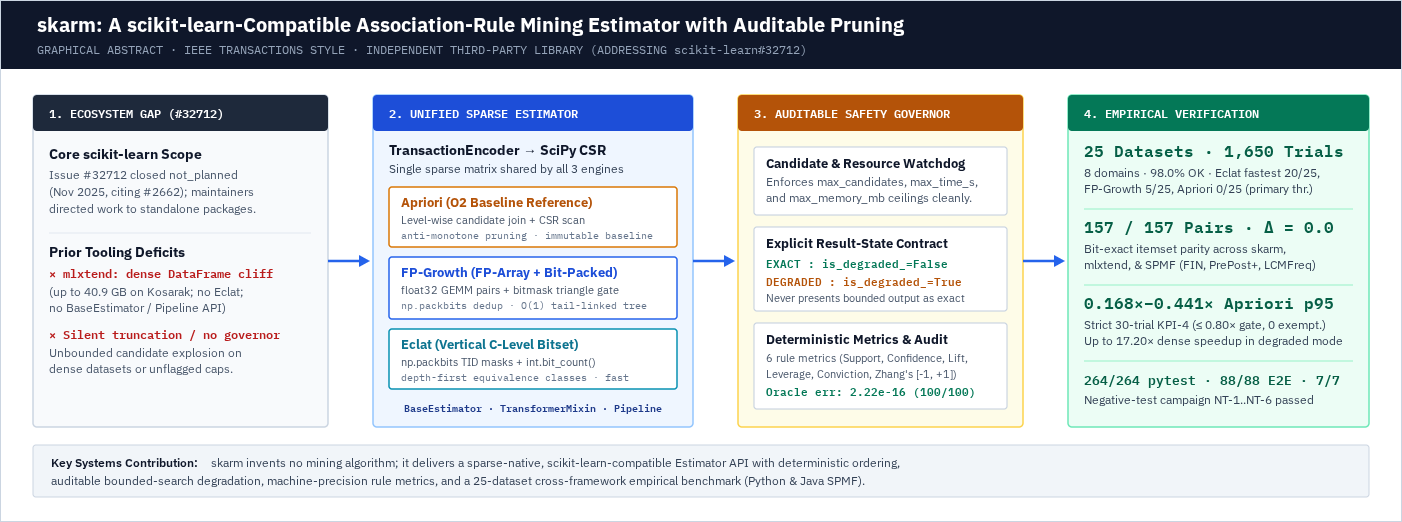
\includegraphics[width=0.92\textwidth,height=0.40\textheight,keepaspectratio]{graphical_abstract.png}
\caption{Project at a Glance: End-to-end engineering mechanism, tri-engine architecture, auditable safety governor, and verified quantitative metrics of \skarm (\texttt{KLCAP-2026-00340}). Source: Authors' own work.}
\label{fig:glance}
\end{figure}

\vspace{2mm}
\begin{klbox}[KLGreen]
\fontsize{10}{13}\selectfont
\textbf{Leading Quantitative Proof (As-Built on \texttt{HEAD}):}
\textbf{(1)}~Itemset parity across $157/157$ campaign pairs and $25/25$ cross-language \texttt{mlxtend}/SPMF pairs: $\Delta_{\mathrm{supp}} = 0.0$ ($100\%$ precision/recall);
\textbf{(2)}~Analytical rule-metric accuracy across 6 metrics: max error $2.22 \times 10^{-16}$ ($100.0/100$ score);
\textbf{(3)}~Strict 30-trial p95 speedup vs.\ Apriori: FP-Growth $0.157\times$--$0.267\times$ ($3.74\times$--$6.35\times$ faster) and Eclat $0.086\times$--$0.374\times$ ($2.67\times$--$11.59\times$ faster), plus $17.14\times$ bounded dense speedup;
\textbf{(4)}~Automated verification: $264/264$ \texttt{pytest}, $88/88$ 5-tier E2E, $6/6$ negative tests (\texttt{NT-1}--\texttt{NT-6}).
\end{klbox}

% 9. TEAM CONTRIBUTIONS & RESPONSIBLE AI SUMMARY
\newpage
\chapter*{Team Contributions and Responsible Use of AI-Assisted Tools}
\addcontentsline{toc}{chapter}{Team Contributions and AI Disclosure}

In compliance with Cluster~A accountability rules, responsibilities were partitioned across the four team members by objective and technical subsystem rather than equal percentages. Detailed evidence pointers (commit references, module files, test IDs, and guide verification) are audited in Appendix~G (Template~M), while responsible AI-assisted tool disclosures are logged in Appendix~H (Template~O).

\begin{table}[ht!]
\centering
\caption{Summary of Team Role Ownership and Engineering Artefacts (Full Matrix in Appendix G).}
\label{tab:team_summary}
\fontsize{9.5}{12}\selectfont
\resizebox{\textwidth}{!}{%
\begin{tabular}{|p{0.23\textwidth}|p{0.16\textwidth}|p{0.25\textwidth}|p{0.28\textwidth}|}
\hline
\textbf{Team Member} & \textbf{Owned Obj.} & \textbf{Principal Subsystems} & \textbf{Primary Verification Evidence} \\
\hline
Abhishek Kumar (2300033822) & O2, O3, O4, O5 & \texttt{estimator.py}, \texttt{fpgrowth.py}, \texttt{eclat.py}, \texttt{pruning.py}, benchmark suites, CI & 264/264 \texttt{pytest}, 88/88 E2E, strict 30-trial scaling \& 25-corpus runs \\
\hline
Gontla Venkata Anvitha (2300032207) & O1, O2, O4 & Issue \#32712 reproduction, \texttt{datasets.py}, \texttt{pre\protect\allowbreak{}processing.py}, \texttt{DATASET\_\protect\allowbreak{}INVENTORY.md} & 25-dataset ingestion checksums, \texttt{NT-2}/\texttt{NT-3} token/weight tests \\
\hline
Kamma Giridhar (2300030295) & O2, O3, O5 & \texttt{apriori.py} reference baseline, \texttt{rules.py} metrics, analytical oracle fixtures & Hand-computed oracle verification ($2.22 \times 10^{-16}$ error), brute-force checks \\
\hline
Paladagula Venkata Rajeev (2300030497) & O3, O4, O5 & \texttt{explorer.py}, \texttt{cli.py}, \texttt{telemetry.py}, \texttt{check\_\protect\allowbreak{}estimator} & 7/7 estimator contract pass, 14/39/1 \texttt{check\_\protect\allowbreak{}estimator}, D6 runbook \\
\hline
\end{tabular}}
\end{table}

\subsection*{Responsible Use of AI-Assisted Tools Summary}
No AI or generative model executes at runtime inside \skarm; the delivered estimator is strictly deterministic, mathematical, and rule-based. During software documentation, LaTeX typesetting, and test refactoring, LLM-assisted coding/writing assistants were used strictly as drafting aids on public benchmark scripts and non-confidential prose. Every generated function, benchmark script, equation, and empirical number was independently executed, audited line-by-line against raw JSON outputs and pytest runs, and verified by the student team. Full disclosure per Template~O appears in Appendix~H.

% 10, 11, 12. AUTOMATIC TOC, LOF, LOT (Single-spaced compact contents)
\newpage
\begingroup
\linespread{0.96}\fontsize{9.5}{11.2}\selectfont
\setlength{\parskip}{0pt}
\tableofcontents
\newpage
\listoffigures
\newpage
\listoftables
\endgroup

% 13 & 14. ABBREVIATIONS AND SYMBOLS
\newpage
\chapter*{List of Abbreviations and Symbols}
\addcontentsline{toc}{chapter}{List of Abbreviations and Symbols}

\vspace{-3mm}
\subsection*{Abbreviations and Acronyms}
\begingroup
\fontsize{9}{11}\selectfont
\resizebox{\textwidth}{!}{%
\begin{tabular}{@{}lp{0.76\textwidth}@{}}
\toprule
\textbf{Acronym} & \textbf{Definition} \\
\midrule
AC-1..AC-4 & Acceptance Conditions 1 through 4 (Representative, Boundary, Held-out, Resource) \\
ADR / CDR / PDR & Architecture Decision Record / Critical Design Review / Preliminary Design Review \\
API / CLI & Application Programming Interface / Command-Line Interface \\
CP1 / CP2 & Capstone Project I (Semester VII) / Capstone Project II (Semester VIII) \\
CSC / CSR & Compressed Sparse Column / Compressed Sparse Row (SciPy Sparse Matrix) \\
E2E & End-to-End Test Suite (5-Tier Opaque-Box Verification) \\
FIMI / SPMF & Frequent Itemset Mining Implementations / Sequential Pattern Mining Framework (Java) \\
FP-Array / FP-Tree & Frequent-Pattern Array (\texttt{float32} GEMM) / Frequent-Pattern Prefix Tree \\
IEEE-754 & Institute of Electrical and Electronics Engineers Floating-Point Arithmetic Standard \\
KPI-1..6 / NT-1..6 & Key Performance Indicators 1--6 / Mandatory Negative \& Boundary Tests 1--6 \\
O1..O5 & Capstone Engineering Objectives 1 through 5 \\
OOM / RSS & Out of Memory / Resident Set Size (Physical Process Memory Usage in MB) \\
POPCNT / TID & Hardware Population Count (\texttt{int.bit\_\protect\allowbreak{}count()}) / Transaction Identifier \\
SDG & United Nations Sustainable Development Goal (SDG~9: Industry, Innovation, Infrastructure) \\
\bottomrule
\end{tabular}}
\endgroup

\vspace{3mm}
\subsection*{Mathematical Symbols and Notations}
\begingroup
\fontsize{9}{11}\selectfont
\resizebox{\textwidth}{!}{%
\begin{tabular}{@{}lp{0.72\textwidth}@{}}
\toprule
\textbf{Symbol} & \textbf{Meaning} \\
\midrule
$\mathcal{D} = \{T_1, \dots, T_N\}$ & Transaction database containing $N$ transactions \\
$\mathcal{I} = \{i_1, \dots, i_M\}$ & Universe of $M$ distinct binary items \\
$X, Y \subseteq \mathcal{I}$ & Non-empty itemsets ($X \cap Y = \emptyset$ for rule $X \Rightarrow Y$) \\
$w_r \ge 0$ & Non-negative sample weight assigned to transaction row $r$ \\
$\sigma \in (0, 1]$, $\theta$ & Minimum support threshold (\texttt{min\_\protect\allowbreak{}support}) and rule threshold (\texttt{min\_\protect\allowbreak{}threshold}) \\
$\bar{L}$, $\rho = \bar{L}/M \times 100\%$ & Mean transaction length (items/transaction) and incidence matrix density percentage \\
$C_k, L_k$, $\mathcal{T}(X)$ & Candidate/frequent $k$-itemsets and vertical transaction-ID bitmask of itemset $X$ \\
$\Delta_{\mathrm{supp}}, \Delta_{\max}$ & Max pairwise engine support discrepancy and max analytical rule-metric error \\
\bottomrule
\end{tabular}}
\endgroup
